\clearpage
\section{Mapa conceptual}

A continuación, se presenta la arquitectura conceptual y evolutiva que sustenta este estudio. El esquema desglosa los antecedentes teóricos fundamentales —desde los modelos empíricos tradicionales y la simulación física en la interfaz urbano-forestal (WUI), hasta las técnicas avanzadas de cuantificación de incertidumbre y computación de alto rendimiento—. Su propósito es ilustrar cómo convergen estos paradigmas para dar solución al vacío de investigación planteado

\begin{figure}[htbp]
    \centering
    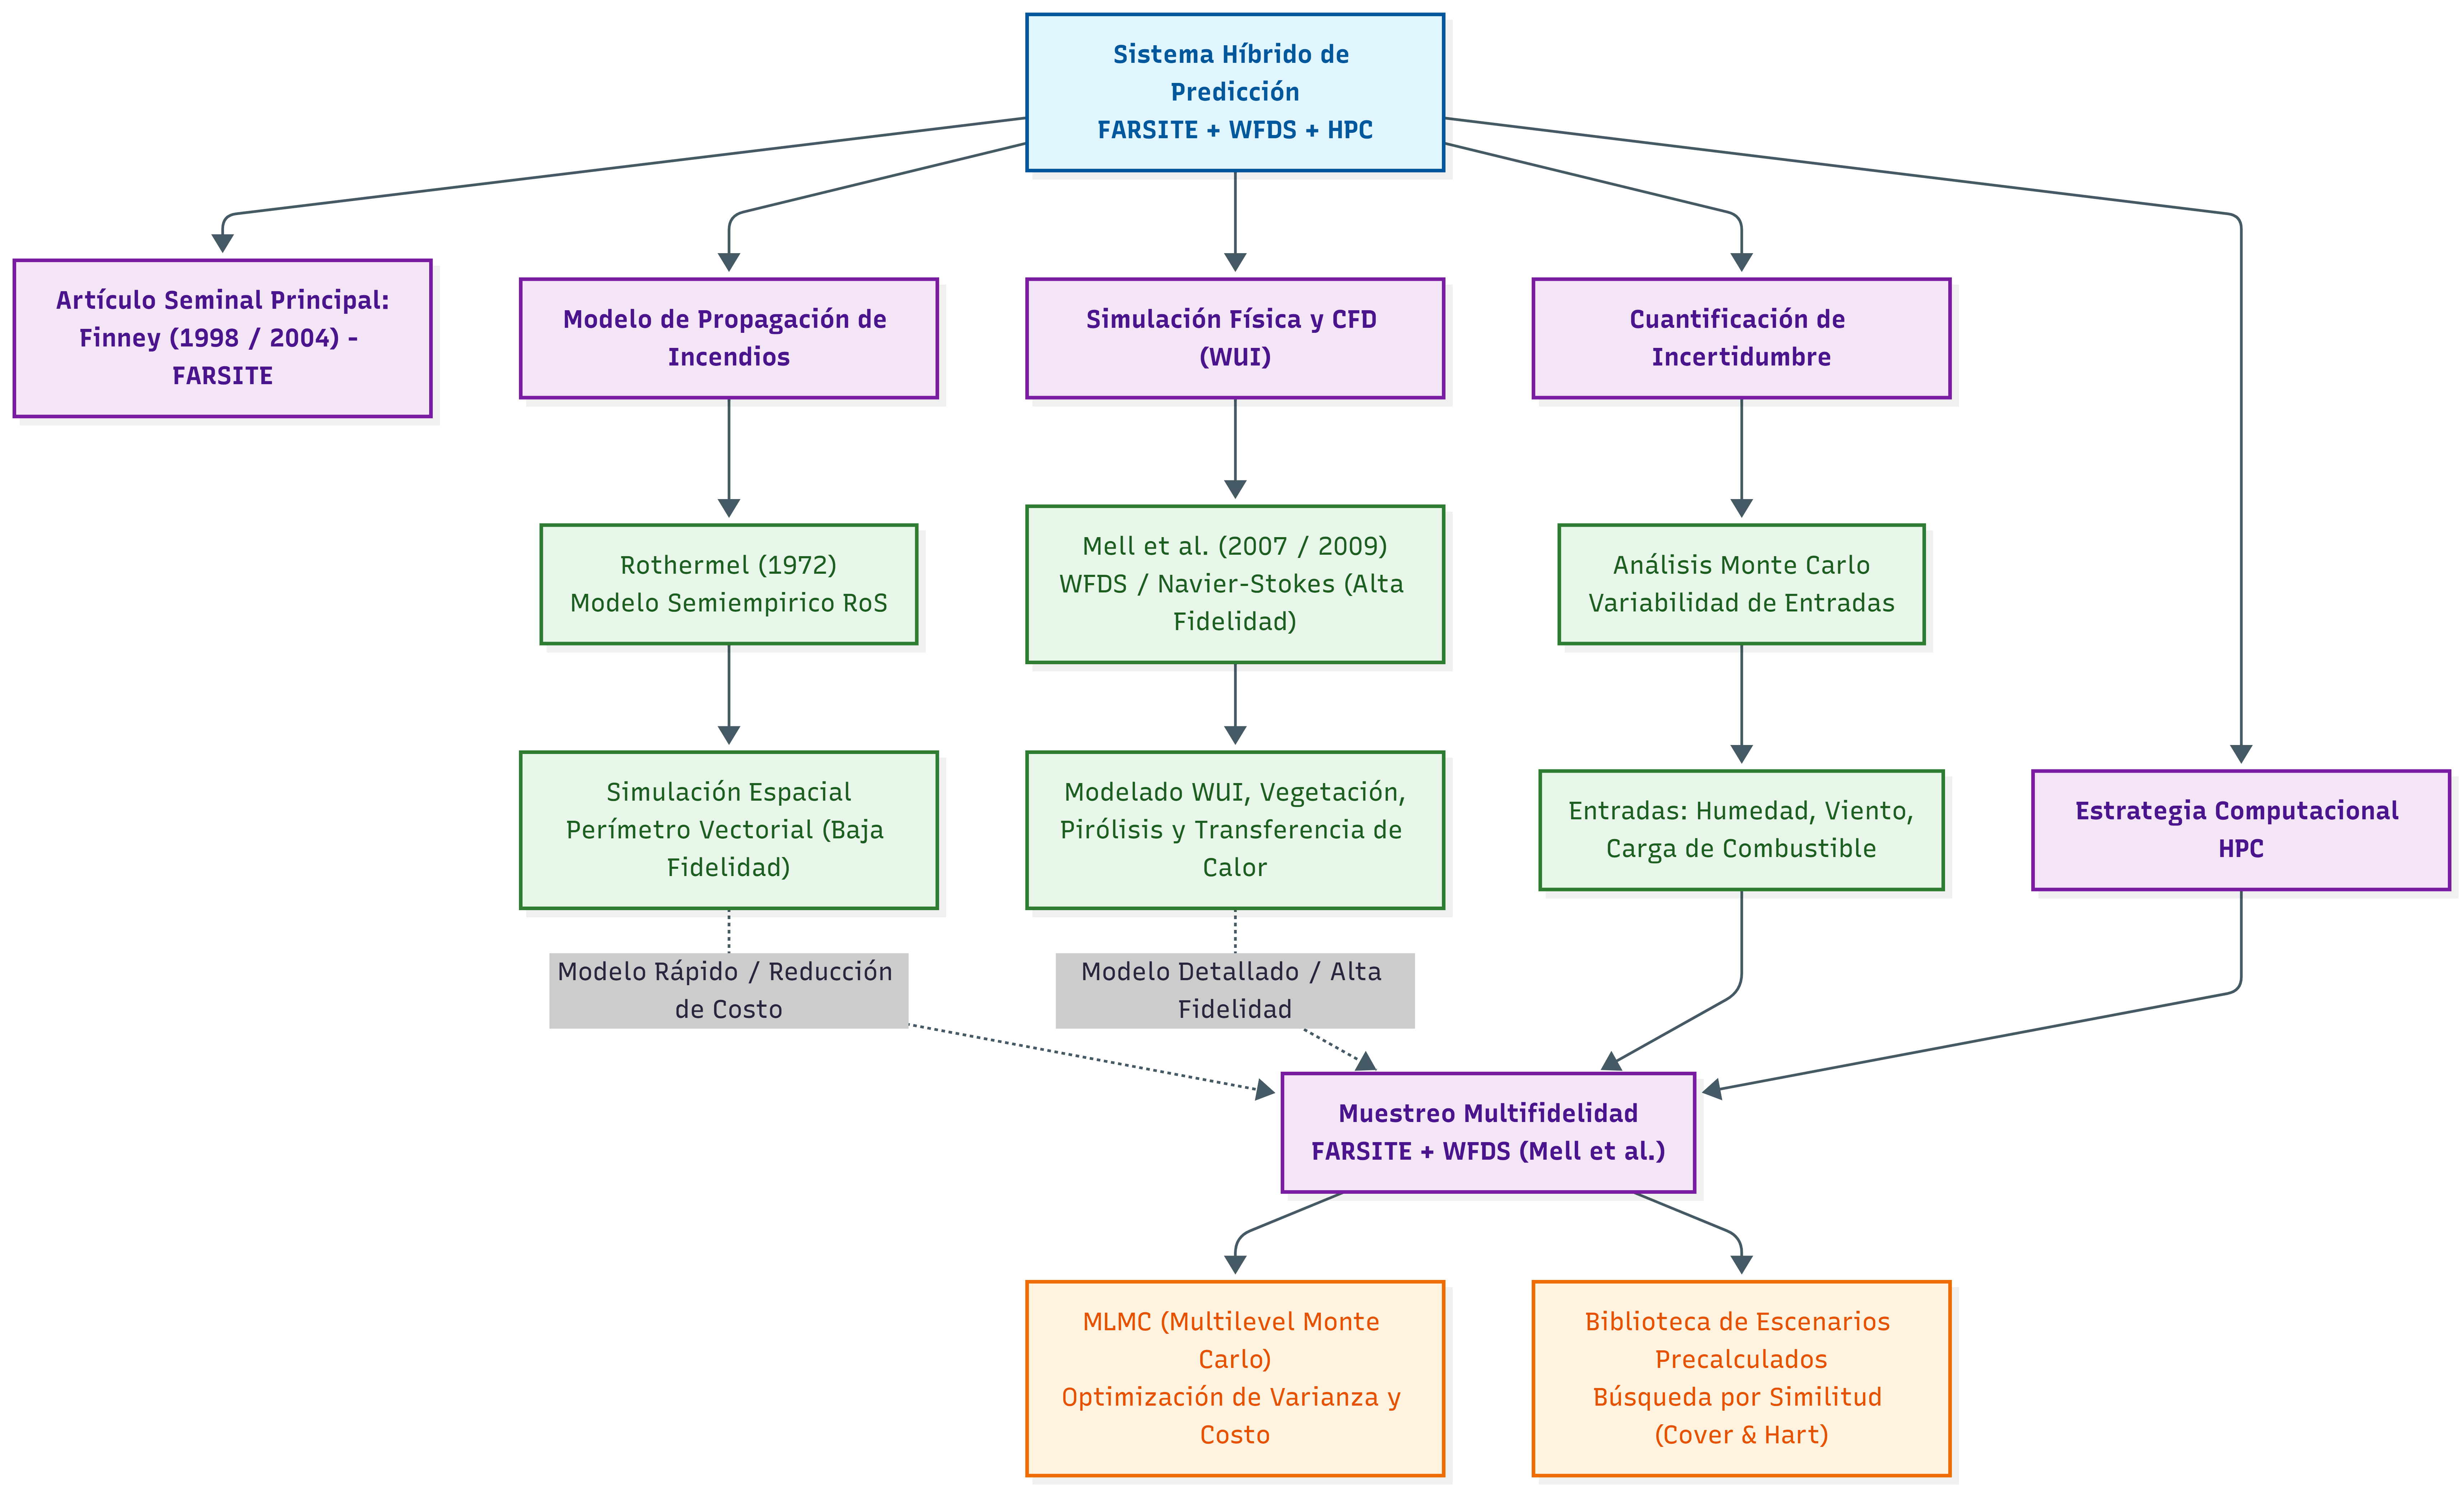
\includegraphics[width=0.95\textwidth]{Mapa-Conceptual}
    \caption{Mapa conceptual de los artículos seminales y arquitectura del sistema de predicción.}
    \label{fig:mapa_conceptual}
\end{figure}